\section{Supplementary Material}
\beginsupplement

\hypertarget{an-example-of-model-non-linearity-in-the-presence-of-a-linear-predictor.}{%
\section{An example of model non-linearity in the presence of a linear
predictor.}\label{an-example-of-model-non-linearity-in-the-presence-of-a-linear-predictor.}}

Notebook available on-line:
https://github.com/spisakt/mlconfound\_manuscript/tree/main/simulated/normality\_and\_linearity\_violation.ipynb

\begin{Shaded}
\begin{Highlighting}[]
\ImportTok{import}\NormalTok{ numpy }\ImportTok{as}\NormalTok{ np}
\ImportTok{import}\NormalTok{ seaborn }\ImportTok{as}\NormalTok{ sns}
\ImportTok{import}\NormalTok{ matplotlib.pyplot }\ImportTok{as}\NormalTok{ plt}
\ImportTok{from}\NormalTok{ sklearn.linear_model }\ImportTok{import}\NormalTok{ Ridge}
\NormalTok{sns.}\BuiltInTok{set}\NormalTok{(rc}\OperatorTok{=}\NormalTok{\{}\StringTok{"figure.figsize"}\NormalTok{:(}\DecValTok{6}\NormalTok{, }\DecValTok{2}\NormalTok{)\})}
\NormalTok{sns.set_style(}\StringTok{"white"}\NormalTok{)}
\end{Highlighting}
\end{Shaded}

\hypertarget{five-features-one-linear-four-sigmoid}{%
\subsubsection{Five features: one linear, four
sigmoid}\label{five-features-one-linear-four-sigmoid}}

\begin{Shaded}
\begin{Highlighting}[]
\NormalTok{n}\OperatorTok{=}\DecValTok{300}
\NormalTok{p}\OperatorTok{=}\DecValTok{5}
\NormalTok{rng }\OperatorTok{=}\NormalTok{ np.random.default_rng(}\DecValTok{42}\NormalTok{)}
\NormalTok{y }\OperatorTok{=}\NormalTok{ np.arange(n)}
\NormalTok{y }\OperatorTok{=}\NormalTok{ (y }\OperatorTok{-}\NormalTok{ y.mean())}\OperatorTok{/}\NormalTok{y.std()}

\NormalTok{X_true }\OperatorTok{=}\NormalTok{ np.repeat(y, p).reshape(n,p)}
\ControlFlowTok{for}\NormalTok{ i }\KeywordTok{in} \BuiltInTok{range}\NormalTok{(}\DecValTok{1}\NormalTok{,}\DecValTok{4}\NormalTok{):}
\NormalTok{    X_true[:,i] }\OperatorTok{=}\NormalTok{ np.tanh(X_true[:,i]}\OperatorTok{*}\DecValTok{2}\NormalTok{)}

\NormalTok{X}\OperatorTok{=}\NormalTok{X_true }\OperatorTok{+}\NormalTok{ rng.normal(}\DecValTok{0}\NormalTok{,}\FloatTok{0.1}\NormalTok{, (n,p))}

\ControlFlowTok{for}\NormalTok{ i }\KeywordTok{in} \BuiltInTok{range}\NormalTok{(}\DecValTok{4}\NormalTok{):}
\NormalTok{    sns.lineplot(x}\OperatorTok{=}\NormalTok{y, y}\OperatorTok{=}\NormalTok{X_true[:,i])}
\NormalTok{    sns.scatterplot(x}\OperatorTok{=}\NormalTok{y, y}\OperatorTok{=}\NormalTok{X[:,i])}
\NormalTok{    plt.show()}
\end{Highlighting}
\end{Shaded}

\begin{figure}
\centering
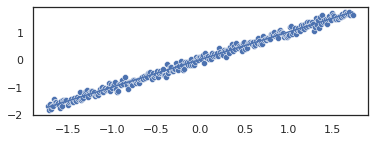
\includegraphics{normality_and_linearity_violation_files/normality_and_linearity_violation_3_0.png}
\caption{png}
\end{figure}

\begin{figure}
\centering
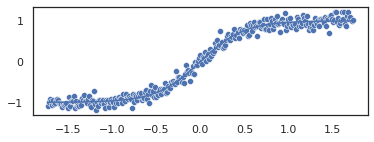
\includegraphics{normality_and_linearity_violation_files/normality_and_linearity_violation_3_1.png}
\caption{png}
\end{figure}

\begin{figure}
\centering
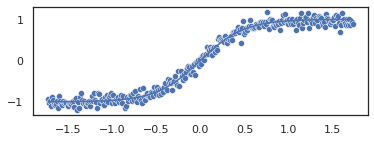
\includegraphics{normality_and_linearity_violation_files/normality_and_linearity_violation_3_2.png}
\caption{png}
\end{figure}

\begin{figure}
\centering
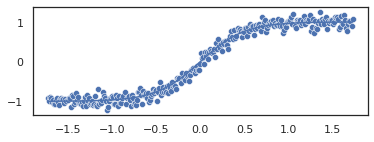
\includegraphics{normality_and_linearity_violation_files/normality_and_linearity_violation_3_3.png}
\caption{png}
\end{figure}

\hypertarget{model-predictions-without-regularization}{%
\subsubsection{\texorpdfstring{Model predictions \textbf{without}
regularization}{Model predictions without regularization}}\label{model-predictions-without-regularization}}

\begin{Shaded}
\begin{Highlighting}[]
\NormalTok{model }\OperatorTok{=}\NormalTok{ Ridge(alpha}\OperatorTok{=}\DecValTok{0}\NormalTok{)}
\NormalTok{model.fit(y}\OperatorTok{=}\NormalTok{y, X}\OperatorTok{=}\NormalTok{X)}
\NormalTok{yhat }\OperatorTok{=}\NormalTok{ model.predict(X)}
\NormalTok{sns.scatterplot(x}\OperatorTok{=}\NormalTok{y, y}\OperatorTok{=}\NormalTok{yhat, alpha}\OperatorTok{=}\FloatTok{0.3}\NormalTok{)}
\CommentTok{#sns.lineplot(x=y, y=y, linestyle="--")}
\NormalTok{model.coef_}
\end{Highlighting}
\end{Shaded}

\begin{verbatim}
array([ 0.47902429,  0.00946499,  0.07378478, -0.02828672,  0.47070535])
\end{verbatim}

\begin{figure}
\centering
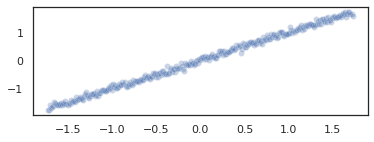
\includegraphics{normality_and_linearity_violation_files/normality_and_linearity_violation_5_1.png}
\caption{png}
\end{figure}

\hypertarget{model-predictions-with-regularization}{%
\subsubsection{\texorpdfstring{Model predictions \textbf{with}
regularization}{Model predictions with regularization}}\label{model-predictions-with-regularization}}

\begin{Shaded}
\begin{Highlighting}[]
\NormalTok{model }\OperatorTok{=}\NormalTok{ Ridge(alpha}\OperatorTok{=}\DecValTok{2000}\NormalTok{)}
\NormalTok{model.fit(y}\OperatorTok{=}\NormalTok{y, X}\OperatorTok{=}\NormalTok{X)}
\NormalTok{yhat }\OperatorTok{=}\NormalTok{ model.predict(X)}
\NormalTok{sns.scatterplot(x}\OperatorTok{=}\NormalTok{y, y}\OperatorTok{=}\NormalTok{yhat, alpha}\OperatorTok{=}\FloatTok{0.3}\NormalTok{)}
\CommentTok{#sns.lineplot(x=y, y=y, linestyle="--")}
\NormalTok{model.coef_}
\end{Highlighting}
\end{Shaded}

\begin{verbatim}
array([0.09472368, 0.07472972, 0.07338482, 0.07440682, 0.09463765])
\end{verbatim}

\begin{figure}
\centering
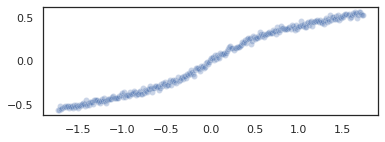
\includegraphics{normality_and_linearity_violation_files/normality_and_linearity_violation_7_1.png}
\caption{png}
\end{figure}

\begin{Shaded}
\begin{Highlighting}[]

\end{Highlighting}
\end{Shaded}



\section{Full confounder test}
\label{sup:full-test}

The full confoudner test generates a null-distribution for an arbitrary predefined test statistic $T(\y,\yhat,\c)$ by sampling permutation based "copies" of $\y$,

$$\y_i^{(j)} \sim Q(\cdot|c_i) \ $$

where, $Q(.|c)$ denotes the conditional distribution of $\y$ given $\c=c$ and $j=1,\dots, m$ indexes the "copy" of $\y$ so that $\y^{(i)} = (y_1^{(j)}, \dots, y_n^{(j)})$ is a permutation of the original vector $\y = (y_1, \dots, y_n)$. This mechanism creates copies $\y^{(1)}, \dots ,\y^{(m)}$ that are exchangeable with the original vector $\y$ under the null hypothesis that $\yhat \independent \y | \c$.

Under the null hypothesis, the triples $$(\y,\yhat,\c), (\y^{(1)}, \yhat, \c),\dots, (\y^{(1)}, \yhat, \c)$$ are all identically distributed and exchangeable, and so are the 
$$T(\y,\yhat,\c), T(\y^{(1)}, \yhat, \c),\dots,T(\y^{(m)}, \yhat, \c)$$
test statistics, as well.

The p-value under the null hypothesis is then obtained as
$$ p= \frac{\sum_{j=1}^m \mathbb{1} \{T(\y^{(j)}, \yhat, \c) \geq T(\y, \yhat, \c) \}  }{m}$$

Let $S_n$ denote the set of all permutations on the indices $\{1,\dots,n\}$ and $\y_\pi = (y_{\pi_1}, \dots, y_{\pi_n})$ the vector $\y$ with its elements reordered according to the permutation $\pi \in S_i$.
The permutation-based copies of $\y$ are then of $\y^{(j)} = \y_{\pi^{(j)}}$ which are drawn so that:

    $$\mathbb{P}(\pi^{(j)} = \pi | \y,\yhat,\c) = \frac{q^n(\y_\pi | \c)}{\sum_{\pi' \in S_n} q^n(\y_{\pi'} | \c)}$$

that is, according to the $q^n(\cdot|\c) := q(\cdot | c_1) \dots q(\cdot|c_n)$ product density corresponding to the conditional distribution $Q(\cdot|\c)$. Note that Eq. \ref{eq-pperm} does not necessarily assume a continuous distribution.
For a verification of the valid type I error control of this approach refer to Theorem 1 in \citep{berrett2020conditional}.



\begin{figure}[H]
  \centering
  \fbox{
   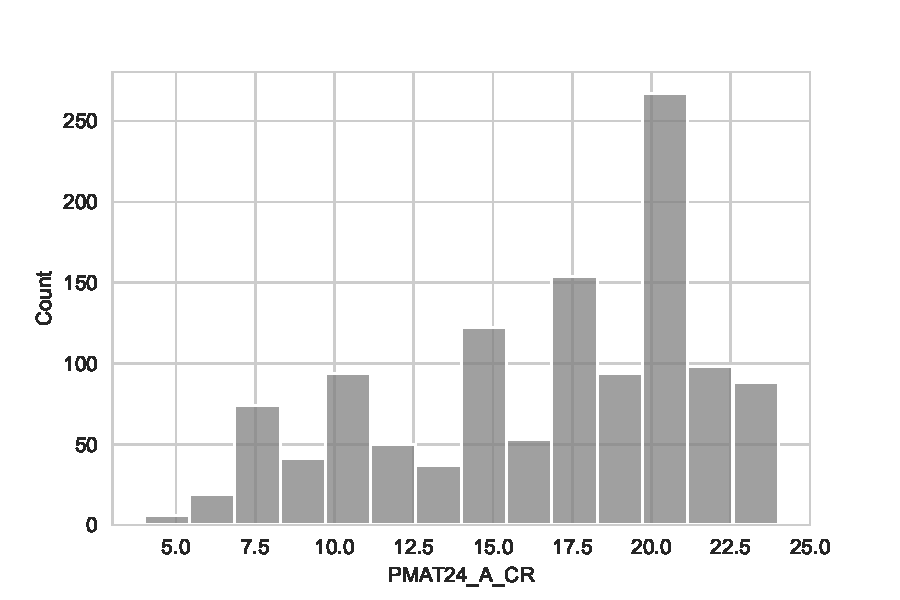
\includegraphics[width=0.36\paperwidth]{fig/supplement/hcp_iq_nonnorm_hist.pdf}
   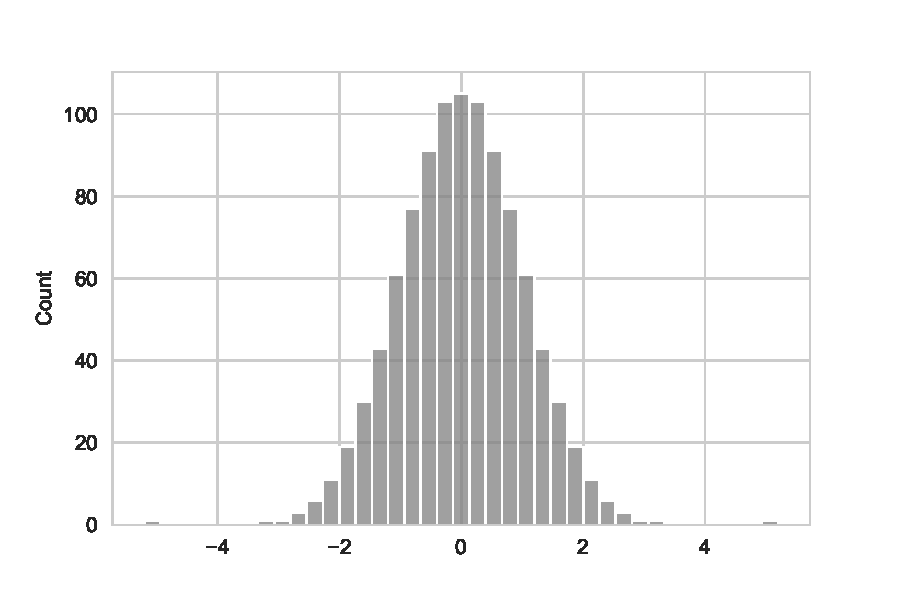
\includegraphics[width=0.36\paperwidth]{fig/supplement/hcp_iq_quanttrf_hist.pdf}
   }
  \caption{Histogram of fluid intelligence score in the HPC dataset, before (left) and after (right) quantile transformation.}
  \label{fig:hcp-hist}
\end{figure}

\begin{figure}[H]
  \centering
  \fbox{
   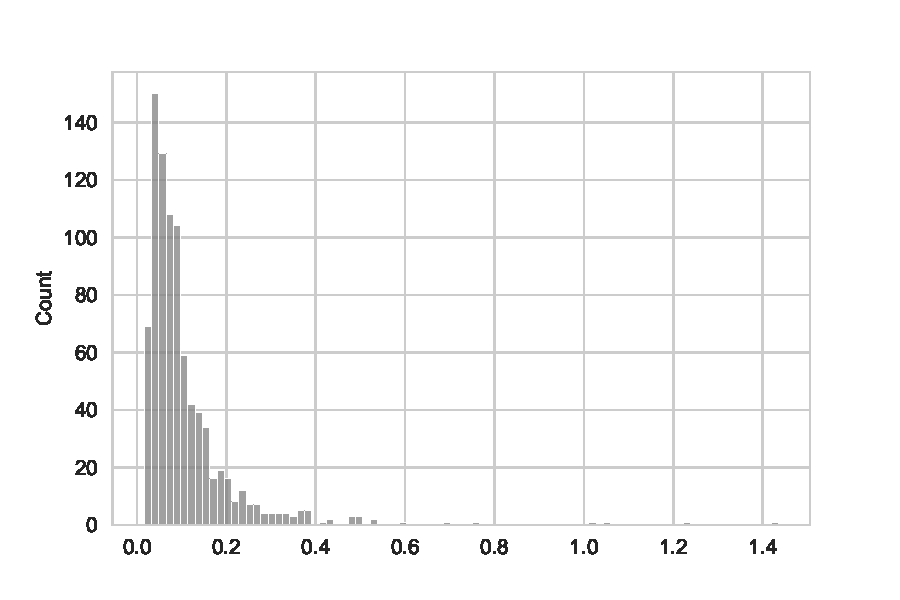
\includegraphics[width=0.36\paperwidth]{fig/supplement/abide_motion_hist.pdf}
   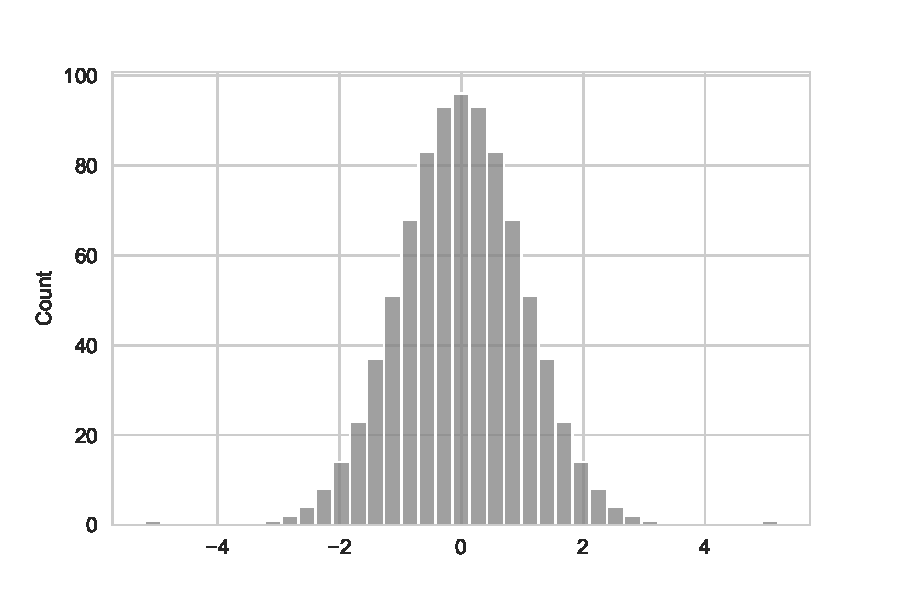
\includegraphics[width=0.36\paperwidth]{fig/supplement/abide_motion_quanttrf_hist.pdf}
   }
  \caption{Histogram of mean framewise displacement in the ABIDE dataset, before (left) and after (right) quantile transformation.}
  \label{fig:abide-hist}
\end{figure}

\begin{figure}[H]
  \centering
  \fbox{
   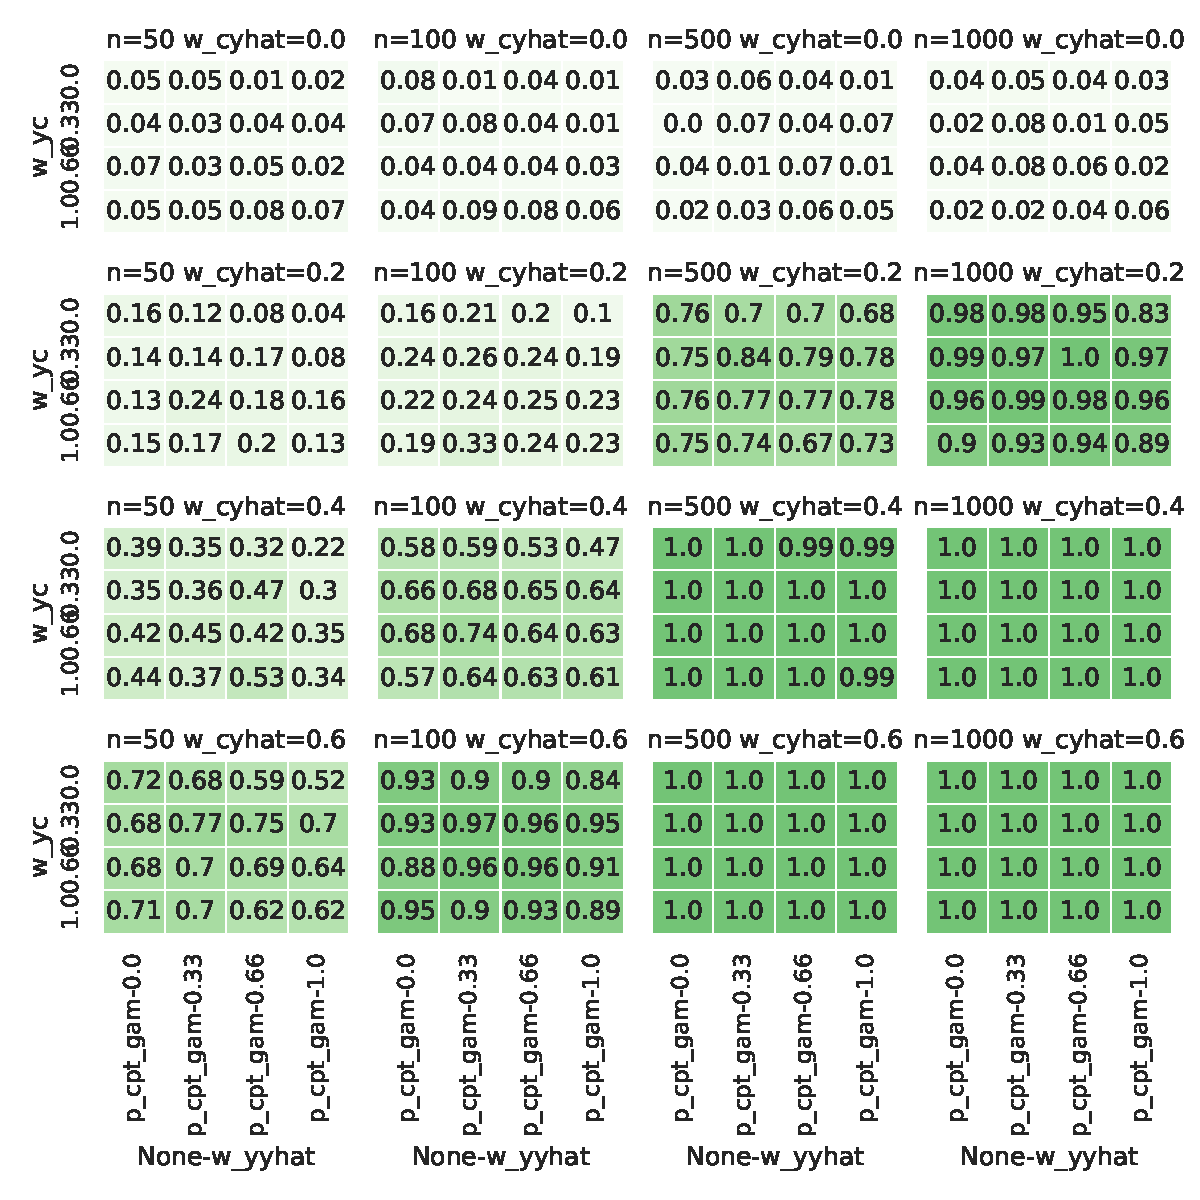
\includegraphics[width=0.75\paperwidth]{fig/raw/sim_h1_ccc_partial_d10e0_sig_cpt_gam.pdf}}
  \caption{Heatmaps showing the positive rates of the 'partial' confounder test, with normal conditional distribution and sigmoid dependence.}
  \label{fig:sim-ccc-sig-partial}
\end{figure}